\documentclass[spanish]{article}
\usepackage[spanish]{babel}
\usepackage{amsmath}
\usepackage{amssymb}
\usepackage[utf8]{inputenc}
\usepackage{vmargin}
\usepackage{graphicx}
\usepackage{wrapfig}
\usepackage[export]{adjustbox}


\begin{document}
	\setpapersize{USletter}
	\setmarginsrb{30mm}{30mm}{30mm}{30mm}{0pt}{0mm}{0pt}{0mm}
	
	\begin{center}
	{ Análisis de Algoritmos, Sem: 2018-1, 3CV2 Práctica 10, 5 de Diciembre del 2017}\\
{ {\bf Práctica 10: Verificación en Tiempo Polinomial}} \\
{ {\bf Martínez Berumen Luis Daniel}} \\

\includegraphics[width=1\textwidth, right]{./imagenes/logos.png}
	\end{center}

	\bigskip
	
	\bigskip
	
	\bigskip
	
	{\LARGE {\bf Abstract}}\\
	
	En esta practica vamos a veirificar si un grafo es o no es un ciclo Hamiltoniano, analizando su tiempo de ejecucion, el cual debe ser polinomial, esto lo explicaremos utilizando graficos y algunos procesos para verificar dichos tiempos, esto es importante ya que, los ciclos Hamiltonianos entran en los problemas del tipo NP, los cuales hemos tratado en la clase.

	\bigskip


	{\Large {\bf Palabras Clave}}\\
	\begin{itemize}
		\item Algoritmo
		\item Hamiltoniano
		\item NP
		\item Grafo
		\item Ciclo
	\end{itemize}
	
	\section{Introducci\'on}
	Un camino hamiltoniano, en el campo matemático de la teoría de grafos, es un camino de un grafo, una sucesión de aristas adyacentes, que visita todos los vértices del grafo una sola vez. Si además el último vértice visitado es adyacente al primero, el camino es un ciclo hamiltoniano.
\newpage
	\section{Conceptos B\'asicos}
	Para la correcta comprension de este trabajo, es necesario definir algunos terminos tales como $\theta$, O y $\Omega$.\\
	 $\theta$(n):\\
		Sea g(n) una función. Se define  $\theta$ (g(n)) como:\\
		
		 	$\theta$(g(n)) = $\{ f(n) \quad | \quad \exists c1,c2>0 \quad \& \quad n_{0}>0 \quad \mid \quad \forall n>=n_{0} \quad 0<= c1g(n) <= f(n) <= c2g(n) \}$
	\bigskip		 	
		 	
	O(n):\\
		Sea  g(n)  una función, O(n) (el pero de los casos) se define como:\\
		
			\hspace{1cm}O(n)=$\{f(n) \quad | \quad \exists c >0 \quad \& \quad n_{0}>0 \quad | \quad f(n) <= Cg(n) \quad \forall  n>= n_{0} \}$
	\bigskip
	
	$\Omega$(n):\\
	Sea  g(n)  una función. Se define $\Omega$ (g(n)) (el mejor de los casos) como:\\

		\hspace{1cm}$\Omega$(g(n)) =$\{f(n) \quad | \quad \exists c >0 \quad \& \quad n_{0}>0 \quad \mid \quad  0<= cg(n)<= f(n) \quad \forall n>= n_{0} \}$
	\bigskip
	
	El algoritmo de encontrar un ciclo Hamiltoniano consiste en cruzar todos los vértices de un grafo sin pasar una segunda vez por alguno de ellos. No obstante, es necesaria otra condición para que dicho camino encontrado sea un ciclo hamiltoniano:

	\begin{center}
		\textit{Un ciclo hamiltoniano es aquella trayectoria donde cruza por todos los vértices del grafo analizado, pero el final de dicho trayecto de terminar en el vértido donde se comenzó. En caso contrario, esta trauectoria se conocerá como Camino Hamiltoniano}
	\end{center}

	A continuación, en la figura 1 se muestra de manera gráfica dicha condición. Podemos tener en un grafo caminos hamiltonianos pero no necesariamente que también sean ciclos hamiltonianos.

	\begin{center}
		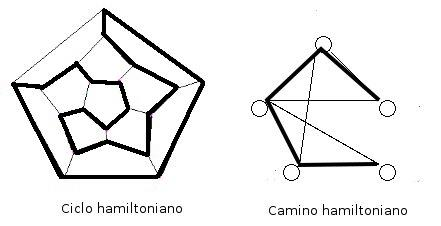
\includegraphics[width=0.55\textwidth]{./imagenes/ciclo_camino_ham.png}\\
		Fig. 1.- Camino Hamiltoniano vs Ciclo Hamiltoniano\\
	\end{center}

	De manera formal, un ciclo Hamiltoniano es necesario que se encuentre en un grafo Hamiltoniano. Éste se puede describir de la siguiente forma:\\
	
	Sea G un grafo conexo. Si existe W $\subset$  V tal que G / W tiene $c$ componentes conexas con c $>$ $|W|$, entonces G no es Hamiltoniano\\

	Para resolver este problema es posible de diferentes maneras. La más rápida de visualizar es por medio de la fuerza bruta, es decir, probar cada combinación entre los vértices del grafo, pero esta solución se vuelve muy lenta; supongamos que tenemos un grafo de n vértices, si se desea realizar todas las combinaciones posibles, tendríamos un total de n!. Como vemos, incrementa factorialmente el tiempo de ejecución por medio de la fuerza bruta. \\	
	
	\newpage	

	Por este motivo, dicho problema se encuentra en la categoría de NP; aunque el incremento de vértices sea pequeño, el tiempo de ejecución crecerá enormemente. Es cierto que hay otros algoritmos que reducen  dicho tiempo, como es el caso del algoritmo de Bellman, Held y Karp, donde usan programación dinámica y el tiempo es de O($n^2$$2n$). Aún con algoritmos con menor tiempo, éstos siguen siendo de carácter exponensial, que para nuestros propósitos sigue teniendo una tasa de crecimiento alta.

	\section{Experimentaci\'on y Resultados}
		
	\subsection{Implemente el algortimo de Verificación de Hamilton que verifique en tiempo polinomial que el certificado C  es o no un ciclo Hamiltoniano del grafo G}

	{\large{ {\bf i) Mediante gráficas, muestre que el certificado es o no un ciclo Hamiltoniano en tiempo polinomial.}}}\\

\begin{center}
		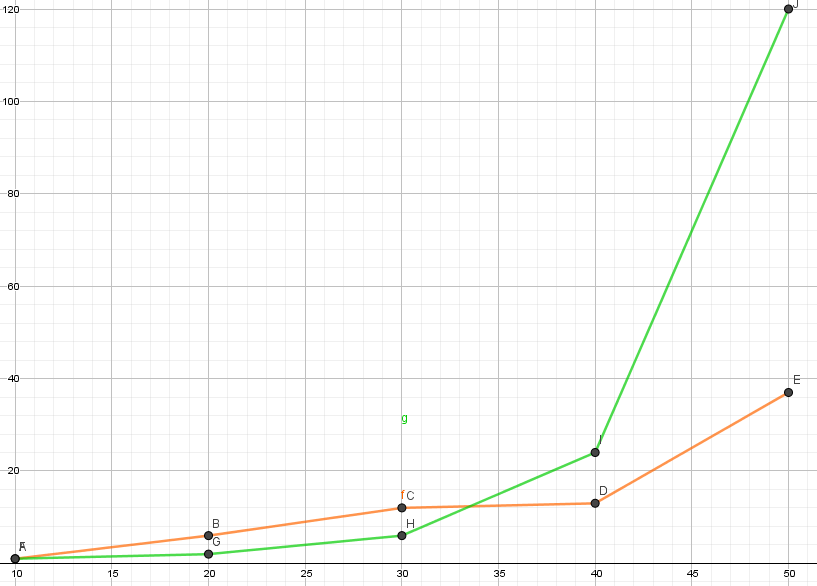
\includegraphics[width=0.55\textwidth]{./imagenes/grafica.png}\\
		Fig. 2.-Resultados\\
	\end{center}

Debido  a  que  el  algoritmo  se  basa  en  la  solucíon  por  fuerza  bruta,  utilizamos  a  O(n!)  como cota superior, la cual representamos con la linea verde.La línea naranja coresponde a los datos obtenidos por el algoritmo implementado. Como se puede notar, hay ocasiones donde los datos obtenidos rebasan nuestra cota superior, esto es debido a que la implementación no sigue estrictamente la lógica de la fuerza bruta; se hicieron algunas modificaciones al algoritmo para lograr su funcionamiento. De igualmanera, el análisis del grafo no únicamente dependerá de la cantidad de nodos, minoritariamentetambíen de la cantidad de conexiones que existan entre ellos.
\newpage
	{\large{ {\bf i) Analíticamente, muestre que el certificado es o no un ciclo Hamiltoniano en tiempo polinomial.}}}\\
	

\newpage
	\section{Conclusi\'on}
	Aun no termino de comprender los problemas NP, pero me parece interesante el tipo de "soluciones" que le damos, y lo pongo así porque no podemos encontrar una solucion a este tipo de problemas, por lo que solamente verificamos si nuestro caso a analizar pertenece a este tipo de problemas. esto de verdad estuvo complicado, ya que los ciclos hamiltonianos se me complicaron un poco, logre sacar la practica batallando mucho y variando con el lenguaje ya que por su complejidad me resulta mas sencillo trabajar sobre Java.


	

\newpage
	\section{Bibliografía}
	\begin{itemize}
		\item Brassard, G. (1997). Fundamentos de Algoritmia. España: Ed. Prentice Hall. ISBN 		848966000X
		\item Harel, D. (2004). Algorithmics: The spirit of Computing (3rd. Ed). Estados Unidos de América: Addison
Wesley. ISBN-13: 978-0321117847
	\end{itemize}


\end{document}